\documentclass{standalone}
%
\usepackage{tikz}
\usetikzlibrary{backgrounds}
\usepackage{xcolor}
%
\definecolor{space}{HTML}{1F2C4E}
\definecolor{moon}{HTML}{AFAFAF}
\definecolor{europa}{HTML}{BAC9AF}
\definecolor{ganymede}{HTML}{90816e}
\definecolor{io}{HTML}{be9d36}
\definecolor{callisto}{HTML}{605f54}
%
\usepackage{fontspec}
%\setmainfont{Open Dyslexic}
\setmainfont{Montserrat}
%
\title{Luna e lune di Giove}
\begin{document}
	\tikzset{
		partial ellipse/.style args = {#1:#2:#3}{insert path={+ (#1:#3) arc (#1:#2:#3)}},
	}
	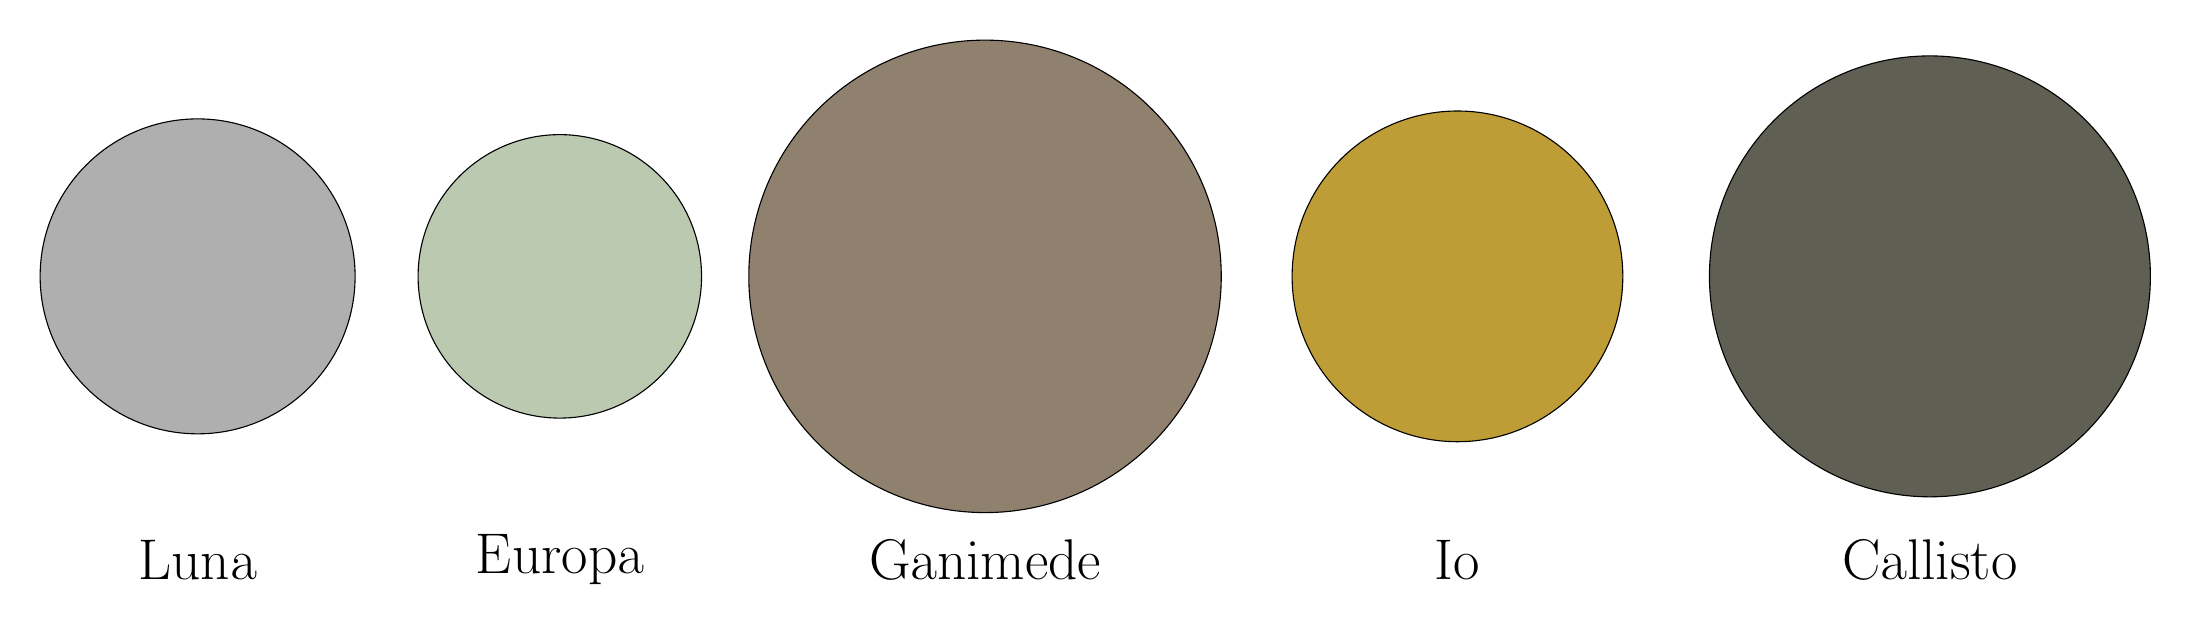
\begin{tikzpicture}[background rectangle/.style={fill=white},show background rectangle,]
		\begin{scope}[scale=2]
			%\draw [fill=space,ultra thick] (17.7,8) rectangle (44,1);
			\coordinate (L) at (0,0);
			\coordinate (E) at (2.3,0);
			\coordinate (G) at (5,0);
			\coordinate (I) at (8,0);
			\coordinate (C) at (11,0);
			\draw [fill=moon] (L) circle (1cm);
			\node at (0,-1.8) {\textcolor{black}{\fontsize{20}{21}\selectfont Luna}};
			\draw [fill=europa] (E) circle (0.9cm);
			\node at (2.3,-1.8) {\textcolor{black}{\fontsize{20}{21}\selectfont Europa}};
			\draw [fill=ganymede] (G) circle (1.5cm);
			\node at (5,-1.8) {\textcolor{black}{\fontsize{20}{21}\selectfont Ganimede}};
			\draw [fill=io] (I) circle (1.05cm);
			\node at (8,-1.8) {\textcolor{black}{\fontsize{20}{21}\selectfont Io}};
			\draw [fill=callisto] (C) circle (1.4cm);
			\node at (11,-1.8) {\textcolor{black}{\fontsize{20}{21}\selectfont Callisto}};
		\end{scope}
	\end{tikzpicture}
\end{document}